% Options for packages loaded elsewhere
\PassOptionsToPackage{unicode}{hyperref}
\PassOptionsToPackage{hyphens}{url}
%
\documentclass[
  11pt,
  ignorenonframetext,
]{beamer}
\usepackage{pgfpages}
\setbeamertemplate{caption}[numbered]
\setbeamertemplate{caption label separator}{: }
\setbeamercolor{caption name}{fg=normal text.fg}
\beamertemplatenavigationsymbolsempty
% Prevent slide breaks in the middle of a paragraph
\widowpenalties 1 10000
\raggedbottom
\setbeamertemplate{part page}{
  \centering
  \begin{beamercolorbox}[sep=16pt,center]{part title}
    \usebeamerfont{part title}\insertpart\par
  \end{beamercolorbox}
}
\setbeamertemplate{section page}{
  \centering
  \begin{beamercolorbox}[sep=12pt,center]{part title}
    \usebeamerfont{section title}\insertsection\par
  \end{beamercolorbox}
}
\setbeamertemplate{subsection page}{
  \centering
  \begin{beamercolorbox}[sep=8pt,center]{part title}
    \usebeamerfont{subsection title}\insertsubsection\par
  \end{beamercolorbox}
}
\AtBeginPart{
  \frame{\partpage}
}
\AtBeginSection{
  \ifbibliography
  \else
    \frame{\sectionpage}
  \fi
}
\AtBeginSubsection{
  \frame{\subsectionpage}
}
\usepackage{amsmath,amssymb}
\usepackage{lmodern}
\usepackage{iftex}
\ifPDFTeX
  \usepackage[T1]{fontenc}
  \usepackage[utf8]{inputenc}
  \usepackage{textcomp} % provide euro and other symbols
\else % if luatex or xetex
  \usepackage{unicode-math}
  \defaultfontfeatures{Scale=MatchLowercase}
  \defaultfontfeatures[\rmfamily]{Ligatures=TeX,Scale=1}
\fi
\usetheme[]{metropolis}
% Use upquote if available, for straight quotes in verbatim environments
\IfFileExists{upquote.sty}{\usepackage{upquote}}{}
\IfFileExists{microtype.sty}{% use microtype if available
  \usepackage[]{microtype}
  \UseMicrotypeSet[protrusion]{basicmath} % disable protrusion for tt fonts
}{}
\makeatletter
\@ifundefined{KOMAClassName}{% if non-KOMA class
  \IfFileExists{parskip.sty}{%
    \usepackage{parskip}
  }{% else
    \setlength{\parindent}{0pt}
    \setlength{\parskip}{6pt plus 2pt minus 1pt}}
}{% if KOMA class
  \KOMAoptions{parskip=half}}
\makeatother
\usepackage{xcolor}
\newif\ifbibliography
\usepackage{graphicx}
\makeatletter
\def\maxwidth{\ifdim\Gin@nat@width>\linewidth\linewidth\else\Gin@nat@width\fi}
\def\maxheight{\ifdim\Gin@nat@height>\textheight\textheight\else\Gin@nat@height\fi}
\makeatother
% Scale images if necessary, so that they will not overflow the page
% margins by default, and it is still possible to overwrite the defaults
% using explicit options in \includegraphics[width, height, ...]{}
\setkeys{Gin}{width=\maxwidth,height=\maxheight,keepaspectratio}
% Set default figure placement to htbp
\makeatletter
\def\fps@figure{htbp}
\makeatother
\setlength{\emergencystretch}{3em} % prevent overfull lines
\providecommand{\tightlist}{%
  \setlength{\itemsep}{0pt}\setlength{\parskip}{0pt}}
\setcounter{secnumdepth}{-\maxdimen} % remove section numbering
\ifLuaTeX
  \usepackage{selnolig}  % disable illegal ligatures
\fi
\IfFileExists{bookmark.sty}{\usepackage{bookmark}}{\usepackage{hyperref}}
\IfFileExists{xurl.sty}{\usepackage{xurl}}{} % add URL line breaks if available
\urlstyle{same} % disable monospaced font for URLs
\hypersetup{
  pdftitle={Análisis de la asociación espacial},
  pdfauthor={Gerardo Martín},
  hidelinks,
  pdfcreator={LaTeX via pandoc}}

\title{Análisis de la asociación espacial}
\subtitle{Interpolación}
\author{Gerardo Martín}
\date{2022-06-29}

\begin{document}
\frame{\titlepage}

\hypertarget{quuxe9-es-la-interpolaciuxf3n}{%
\section{¿Qué es la
interpolación?}\label{quuxe9-es-la-interpolaciuxf3n}}

\begin{frame}{Descripción}
\protect\hypertarget{descripciuxf3n}{}
Procedimiento analítico para predecir variabilidad de proceso espacial a
partir de los valores observados y su ubicación
\end{frame}

\begin{frame}{Diagrama}
\protect\hypertarget{diagrama}{}
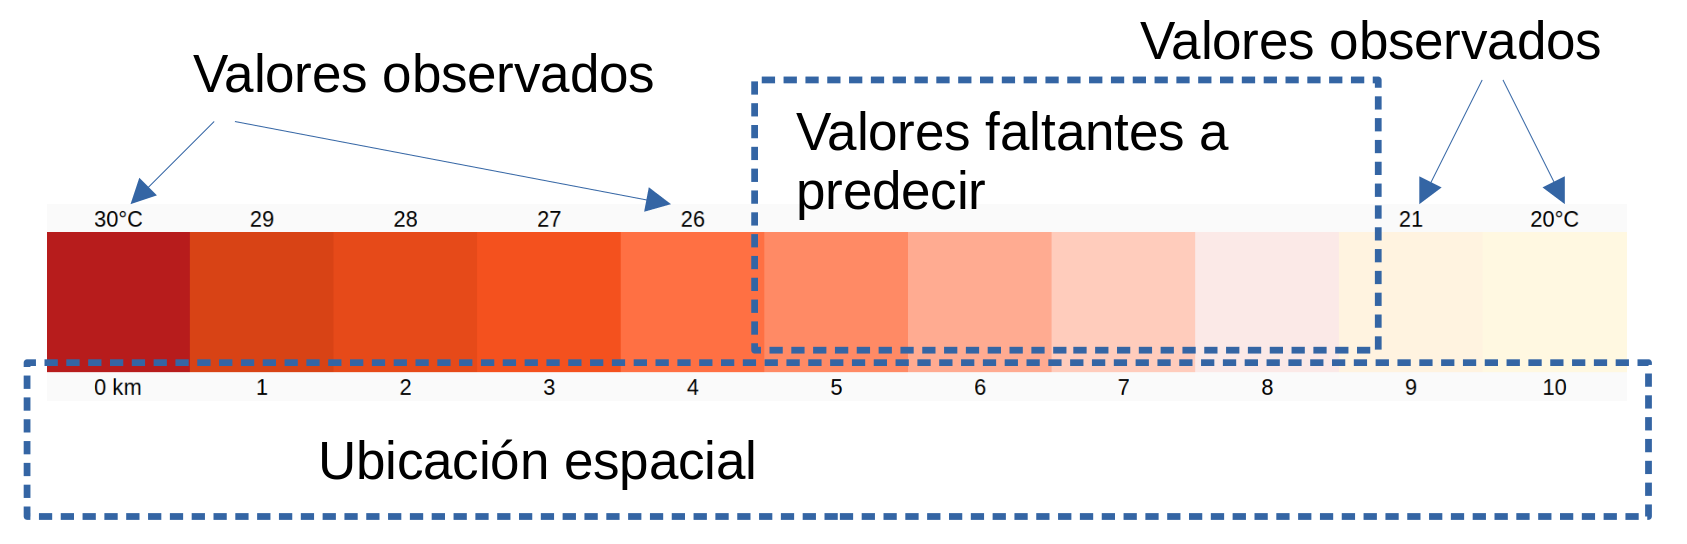
\includegraphics{Interpolacion/Interpolacion}
\end{frame}

\begin{frame}{Ejemplo}
\protect\hypertarget{ejemplo}{}
Variable:

\[X = \{1, 2, , 4, , 6, , , 9 \}\]

Valores faltantes:

\[3, 5, 7\]
\end{frame}

\begin{frame}{Ejemplo en 2 dimensiones}
\protect\hypertarget{ejemplo-en-2-dimensiones}{}
\[\begin{matrix}
1 &   & 3 & 4 \\
  & 2 &   & 5 \\
3 & 4 & 1 & 6 \\
4 &   & 2 & 
\end{matrix}\]
\end{frame}

\begin{frame}{Solución 1}
\protect\hypertarget{soluciuxf3n-1}{}
Hay múltiples soluciones, por ejemplo, promedio de vecinos tipo torre:

\[\begin{matrix}
1 & 2 & 3 & 4 \\
2 & 2 & 2.75 & 5 \\
3 & 4 & 1 & 6 \\
4 & 3.33 & 2 & 4
\end{matrix}\]
\end{frame}

\begin{frame}{Solución 2}
\protect\hypertarget{soluciuxf3n-2}{}
Promedio de vecinos \emph{existentes} tipo reina

\[\begin{matrix}
1 & 2 & 3 & 4 \\
2.4 & 2 & 3.625 & 5 \\
3 & 4 & 1 & 6 \\
4 & 2.8 & 2 & 3
\end{matrix}\]
\end{frame}

\hypertarget{tuxe9cnicas-utilizadas-comunmente}{%
\section{Técnicas utilizadas
comunmente}\label{tuxe9cnicas-utilizadas-comunmente}}

\begin{frame}{Vecino más próximo}
\protect\hypertarget{vecino-muxe1s-pruxf3ximo}{}
Consiste en:

\begin{enumerate}
\tightlist
\item
  Identificar unidades espaciales más cercanas a aquellas donde contamos
  con mediciones
\item
  Asignar a esas unidades espaciales los valores de la unidad cercana
\end{enumerate}
\end{frame}

\begin{frame}{Ejemplo de vecino más próximo}
\protect\hypertarget{ejemplo-de-vecino-muxe1s-pruxf3ximo}{}
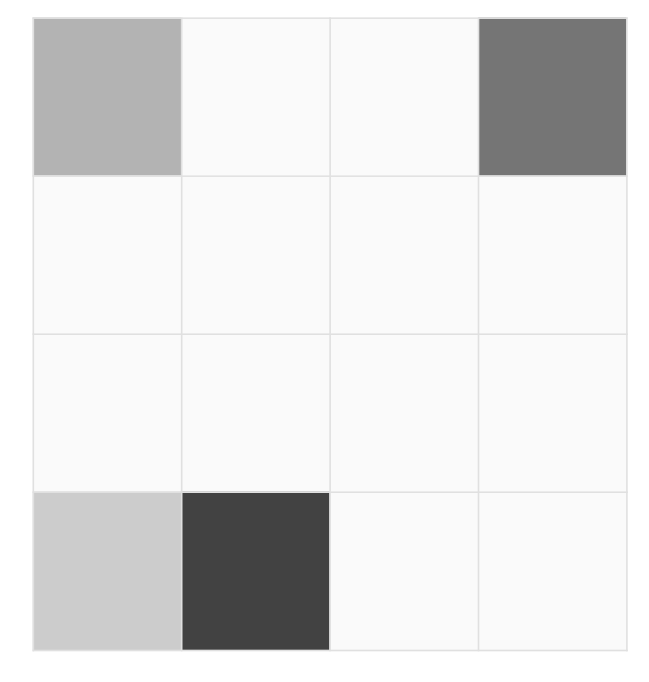
\includegraphics{Interpolacion/Ejemplo-vecino-0.png}
\end{frame}

\begin{frame}{Ejemplo de vecino más próximo}
\protect\hypertarget{ejemplo-de-vecino-muxe1s-pruxf3ximo-1}{}
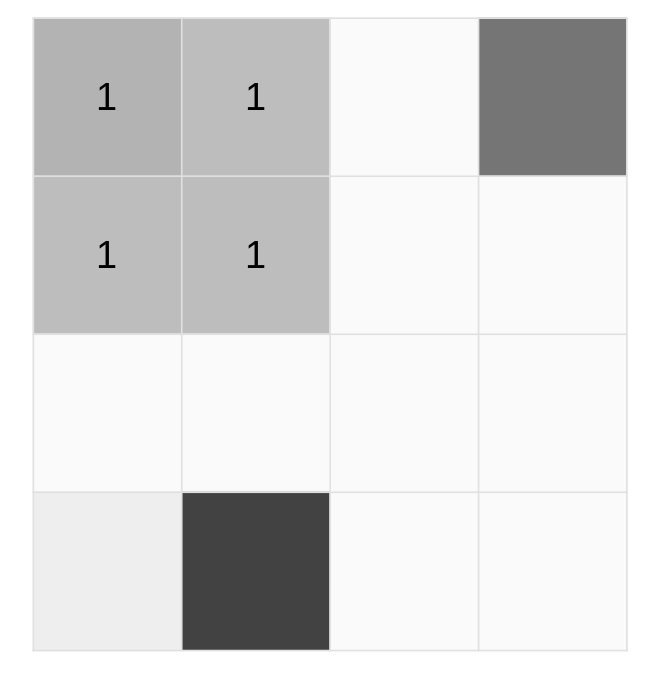
\includegraphics{Interpolacion/Ejemplo-vecino-1.png}
\end{frame}

\begin{frame}{Ejemplo de vecino más próximo}
\protect\hypertarget{ejemplo-de-vecino-muxe1s-pruxf3ximo-2}{}
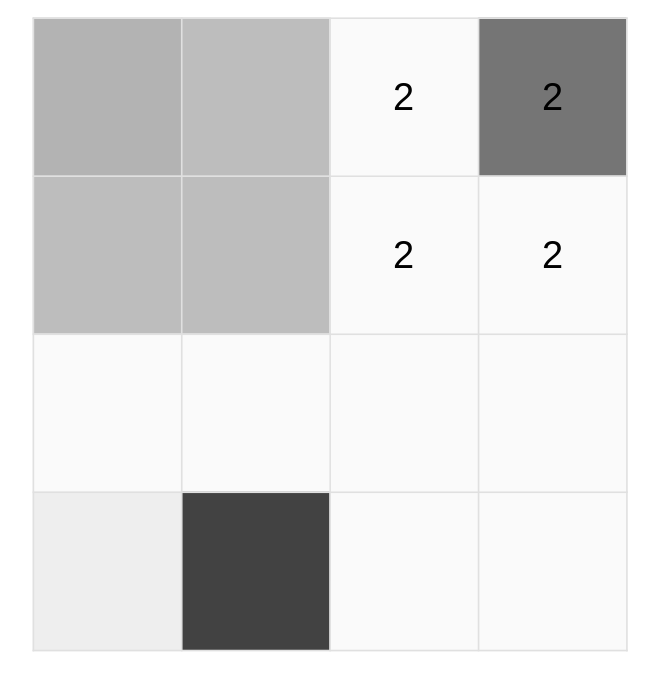
\includegraphics{Interpolacion/Ejemplo-vecino-2.png}
\end{frame}

\begin{frame}{Ejemplo de vecino más próximo}
\protect\hypertarget{ejemplo-de-vecino-muxe1s-pruxf3ximo-3}{}
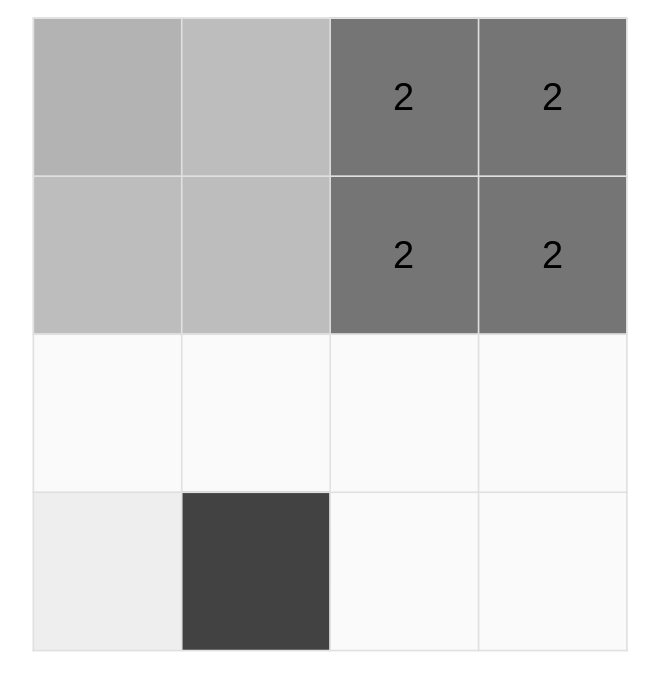
\includegraphics{Interpolacion/Ejemplo-vecino-3.png}
\end{frame}

\begin{frame}{Ejemplo de vecino más próximo}
\protect\hypertarget{ejemplo-de-vecino-muxe1s-pruxf3ximo-4}{}
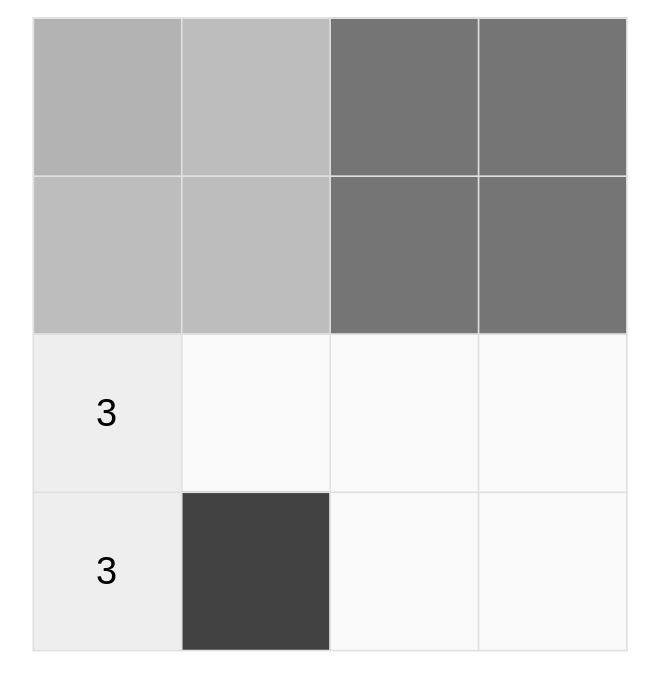
\includegraphics{Interpolacion/Ejemplo-vecino-4.png}
\end{frame}

\begin{frame}{Ejemplo de vecino más próximo}
\protect\hypertarget{ejemplo-de-vecino-muxe1s-pruxf3ximo-5}{}
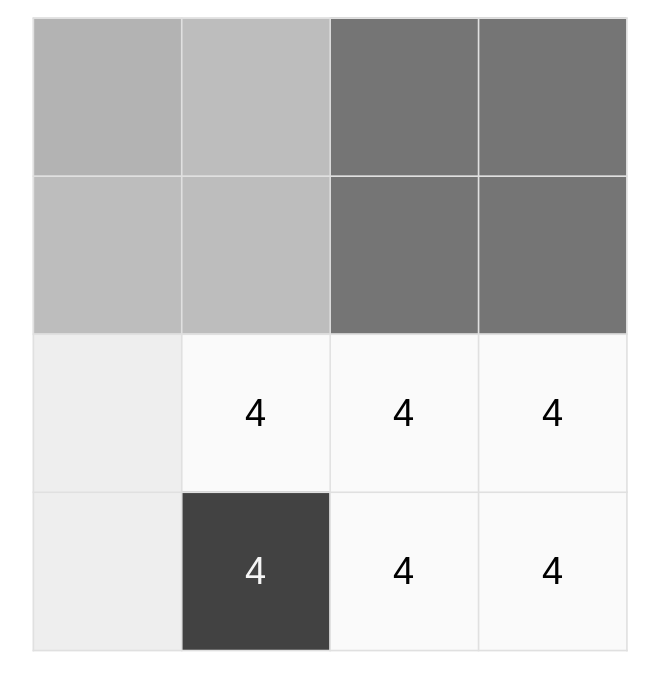
\includegraphics{Interpolacion/Ejemplo-vecino-5.png}
\end{frame}

\begin{frame}{Ejemplo de vecino más próximo}
\protect\hypertarget{ejemplo-de-vecino-muxe1s-pruxf3ximo-6}{}
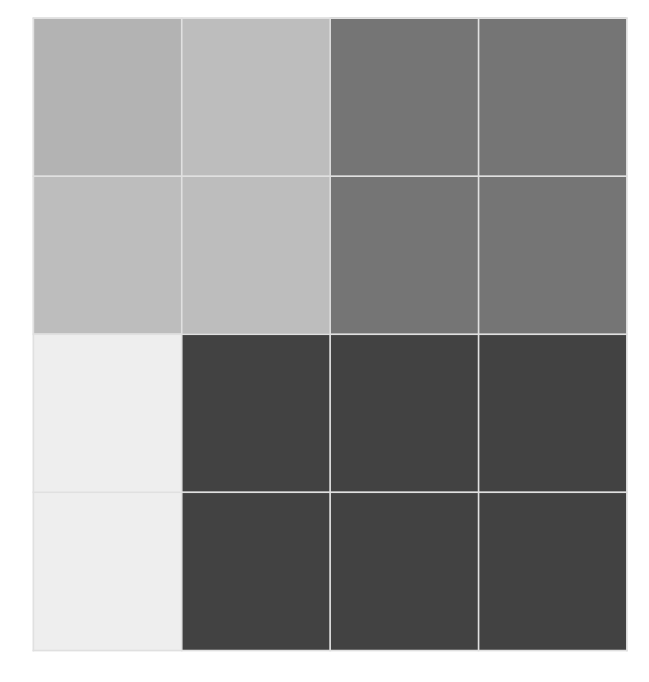
\includegraphics{Interpolacion/Ejemplo-vecino-6.png}
\end{frame}

\begin{frame}{Para muchas unidades espaciales}
\protect\hypertarget{para-muchas-unidades-espaciales}{}
\begin{enumerate}
\tightlist
\item
  Crear teselado
\item
  Asignar valores a cada unidad espacial del teselado
\item
  Rasterizar el teselado
\end{enumerate}
\end{frame}

\begin{frame}{Crear teselado}
\protect\hypertarget{crear-teselado}{}
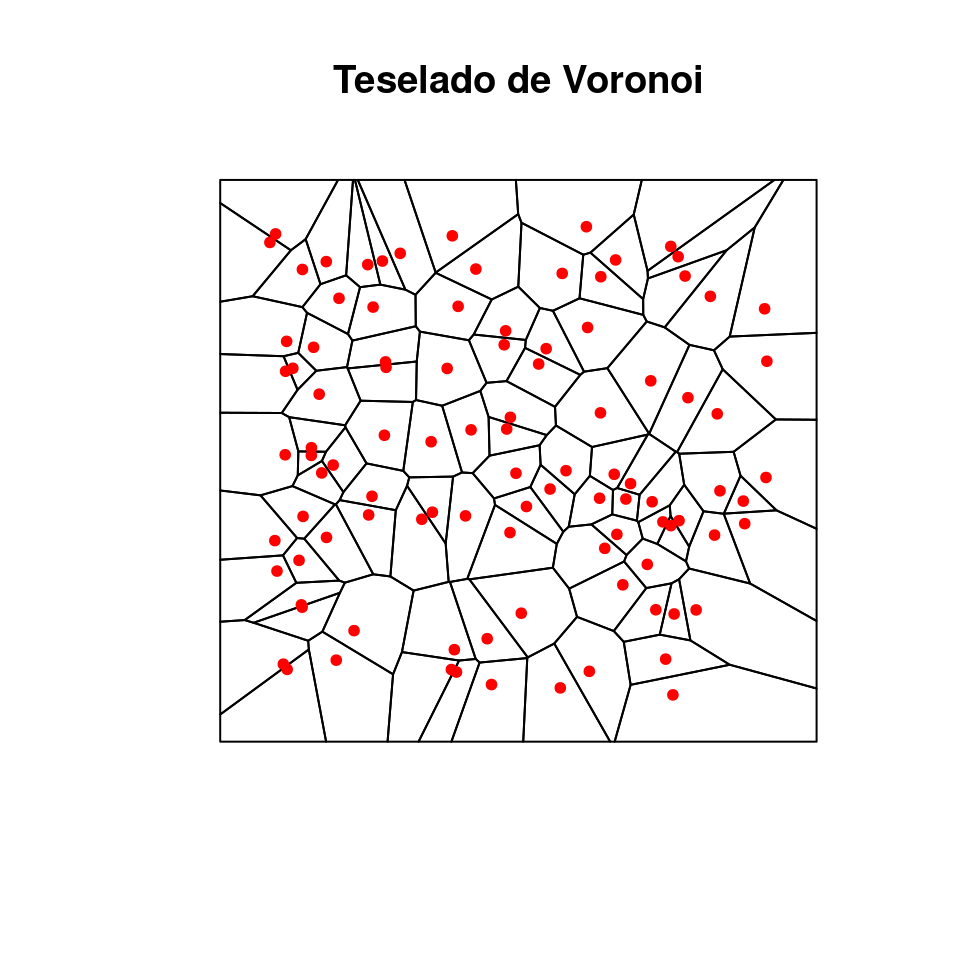
\includegraphics{Interpolacion/Voro-1.png}
\end{frame}

\begin{frame}{El teselado}
\protect\hypertarget{el-teselado}{}
\begin{itemize}
\item
  Genera polígonos alrededor de los puntos de muestreo
\item
  Cualquier punto dentro de los polígonos está más cerca del sitio de
  muestreo adentro que cualquier otro
\end{itemize}
\end{frame}

\begin{frame}{Vista cercana del teselado}
\protect\hypertarget{vista-cercana-del-teselado}{}
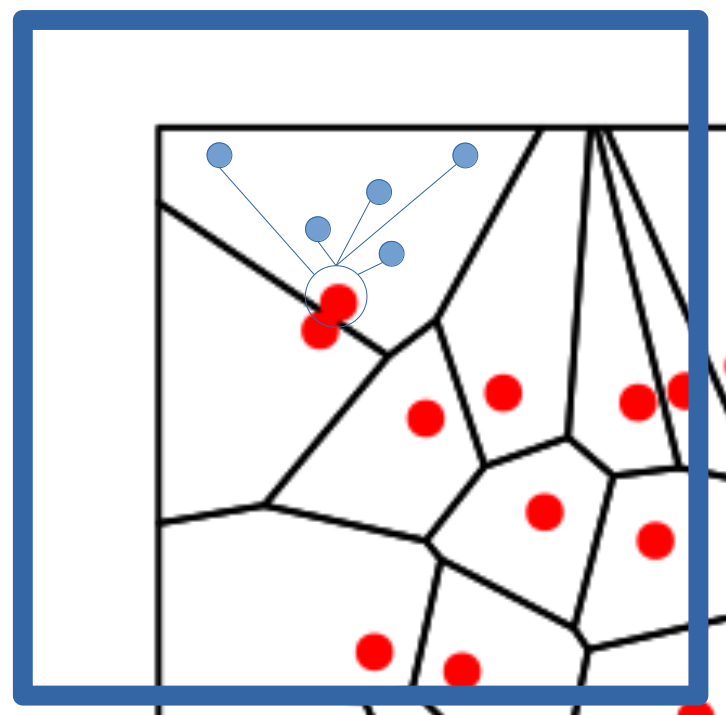
\includegraphics{Interpolacion/Voronoi-cerca-0.png}
\end{frame}

\begin{frame}{Vista cercana del teselado}
\protect\hypertarget{vista-cercana-del-teselado-1}{}
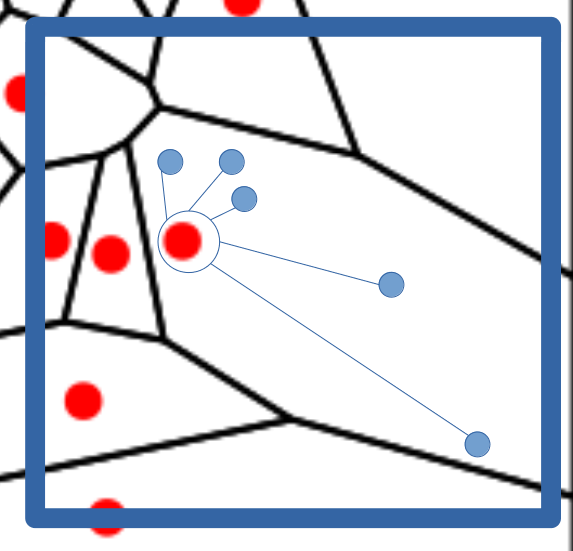
\includegraphics{Interpolacion/Voronoi-cerca-1.png}
\end{frame}

\begin{frame}{Vista cercana del teselado}
\protect\hypertarget{vista-cercana-del-teselado-2}{}
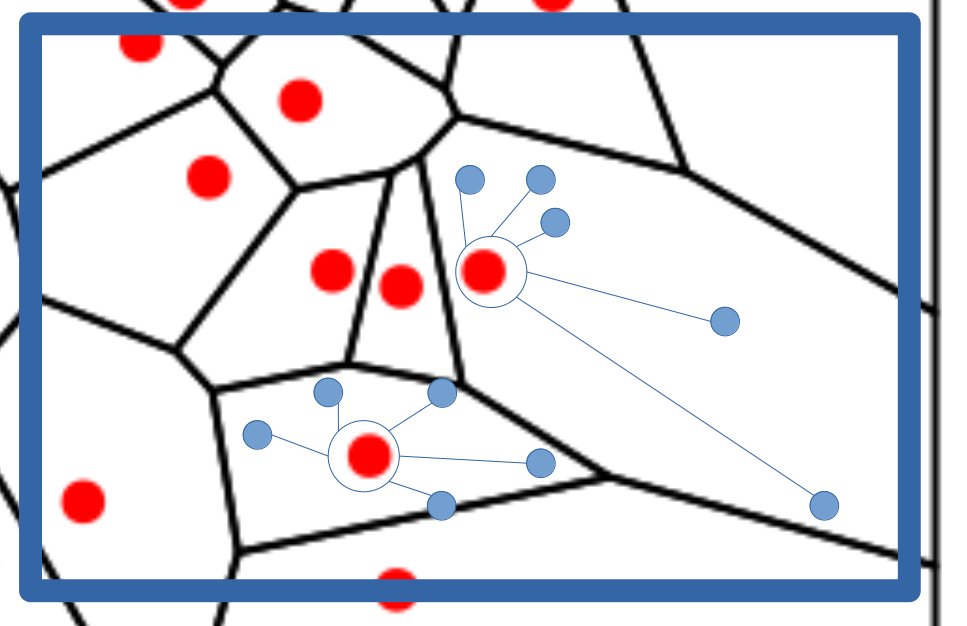
\includegraphics{Interpolacion/Voronoi-cerca-2.png}
\end{frame}

\begin{frame}{La interpolación}
\protect\hypertarget{la-interpolaciuxf3n}{}
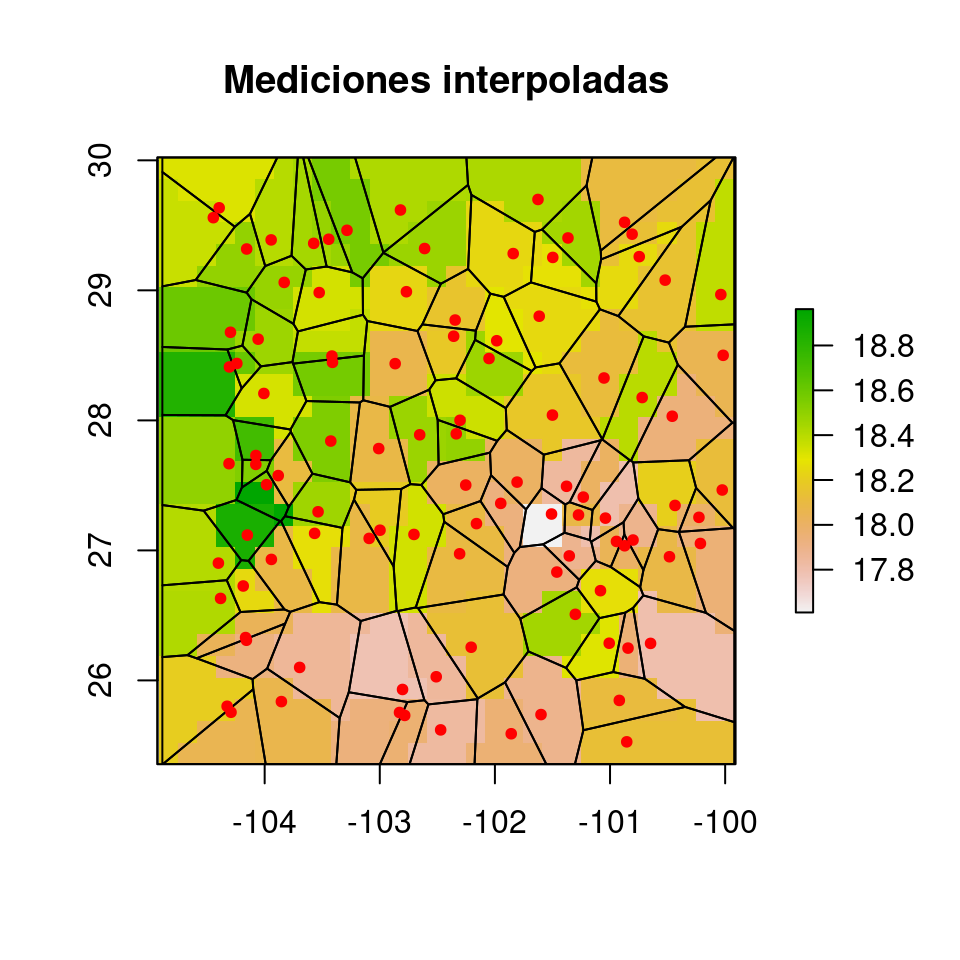
\includegraphics{Interpolacion/Ngb-1.png}
\end{frame}

\hypertarget{otras-metodologuxedas-de-interpolaciuxf3n}{%
\section{Otras metodologías de
interpolación}\label{otras-metodologuxedas-de-interpolaciuxf3n}}

\begin{frame}{Ponderada por inverso de la distancia}
\protect\hypertarget{ponderada-por-inverso-de-la-distancia}{}
\begin{itemize}
\item
  En vecino más próximo se asigna mismo valor que de mediciones
\item
  En inverso de distancia, valor es inversamente proporcional a
  distancia lineal
\end{itemize}
\end{frame}

\begin{frame}{IDW}
\protect\hypertarget{idw}{}
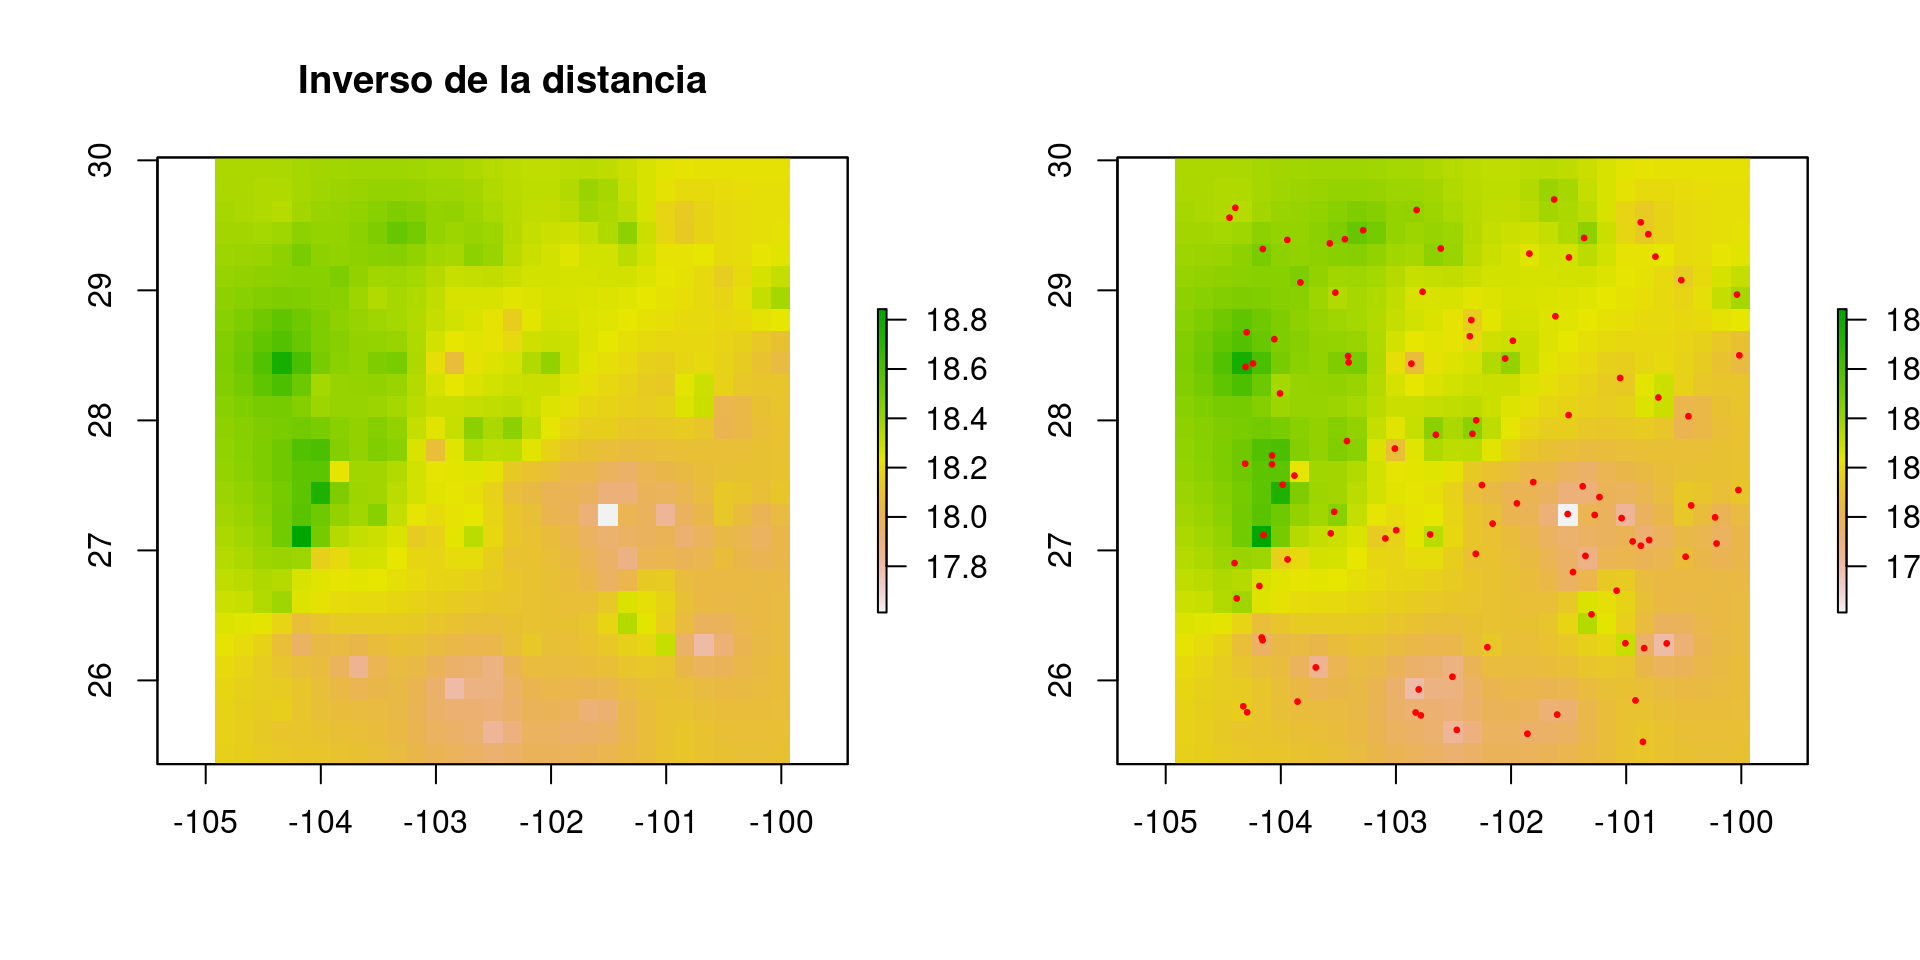
\includegraphics{Interpolacion/Idw-1.png}
\end{frame}

\begin{frame}{Regresión sobre las coordenadas}
\protect\hypertarget{regresiuxf3n-sobre-las-coordenadas}{}
\begin{itemize}
\tightlist
\item
  Valores son función de coordenadas geográficas
\end{itemize}

\[y(Lat, Lon) = \alpha + \beta_1 Lat + \beta_2 Lon\] - \textbf{Sólo
sirve si el gradiente en espacio es lineal}
\end{frame}

\begin{frame}{RSC}
\protect\hypertarget{rsc}{}
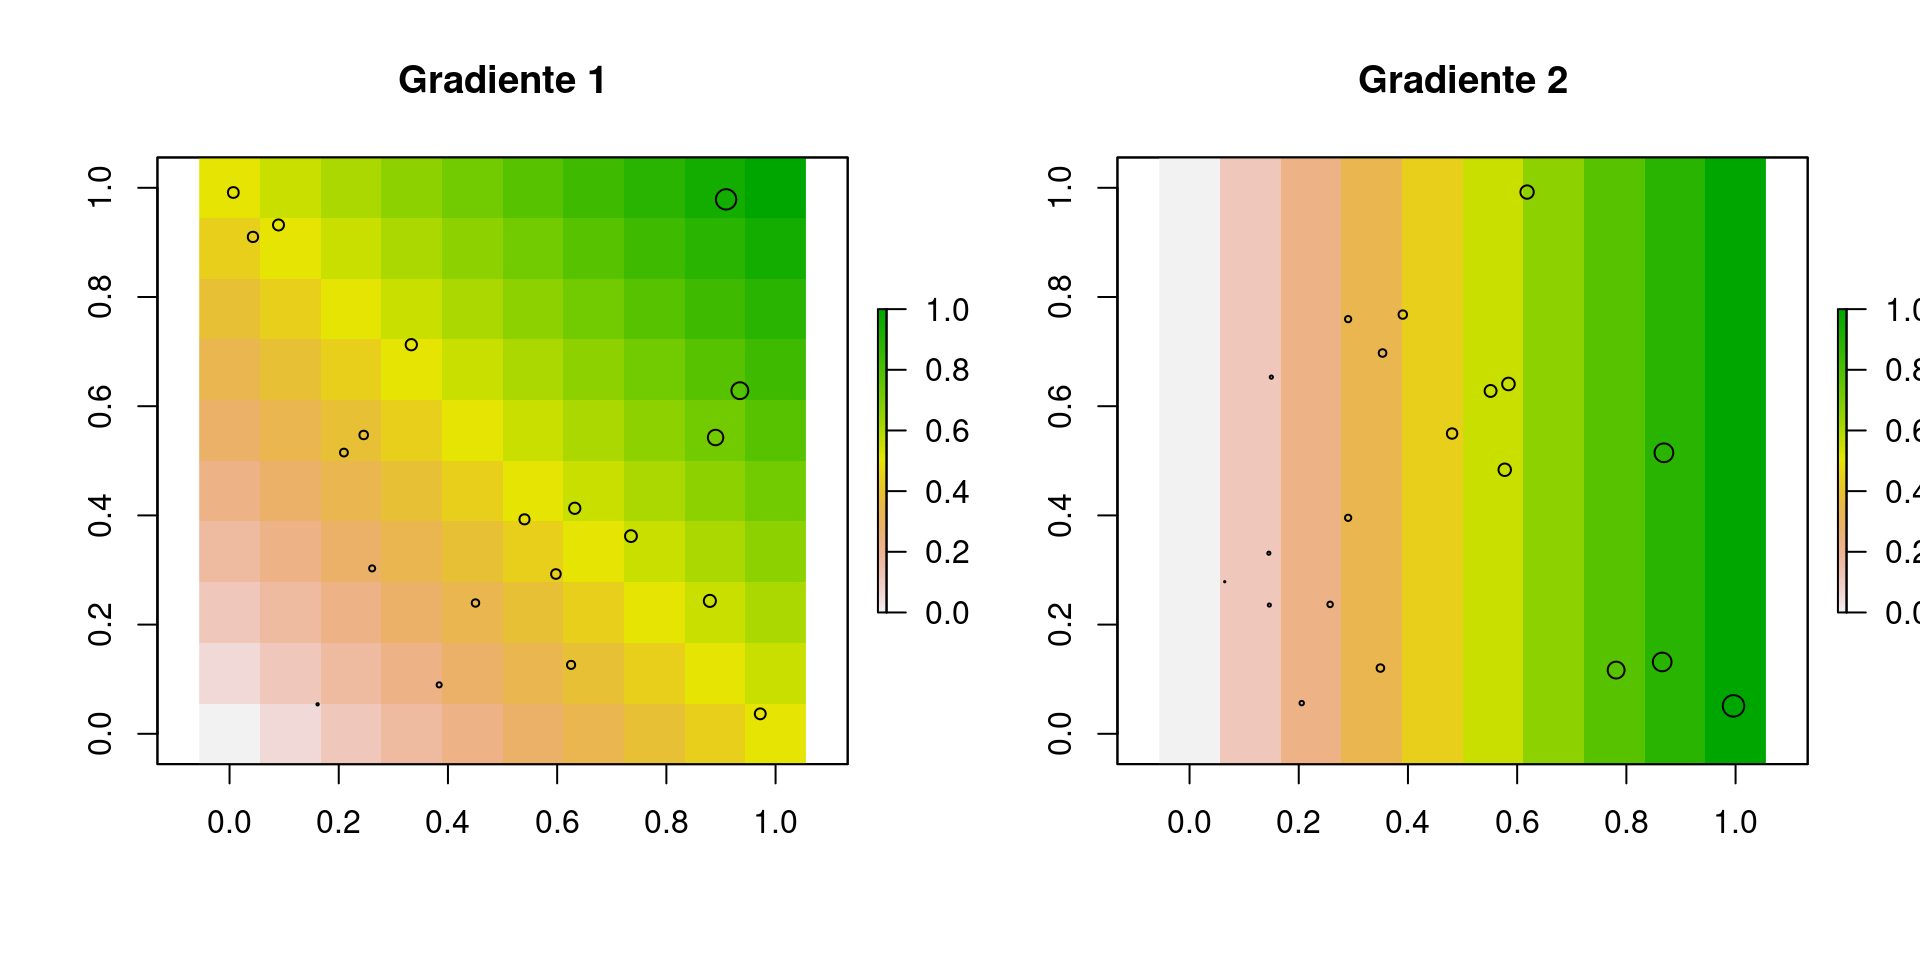
\includegraphics{Interpolacion/Gradientes-1.png}
\end{frame}

\begin{frame}{Splines}
\protect\hypertarget{splines}{}
\begin{itemize}
\item
  Regresión sobre coordenadas, sonde gradiente no es lineal
\item
  Puede ajustar relaciones muy complejas entre variable dependiente e
  independientes
\end{itemize}
\end{frame}

\begin{frame}{Splines - Ejemplo}
\protect\hypertarget{splines---ejemplo}{}
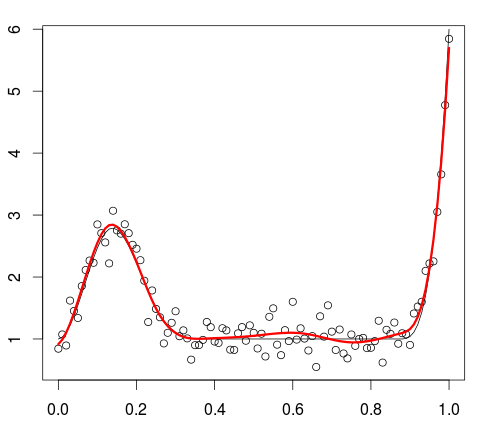
\includegraphics{Interpolacion/Splines.png}
\end{frame}

\begin{frame}{Ejemplo de splines}
\protect\hypertarget{ejemplo-de-splines}{}
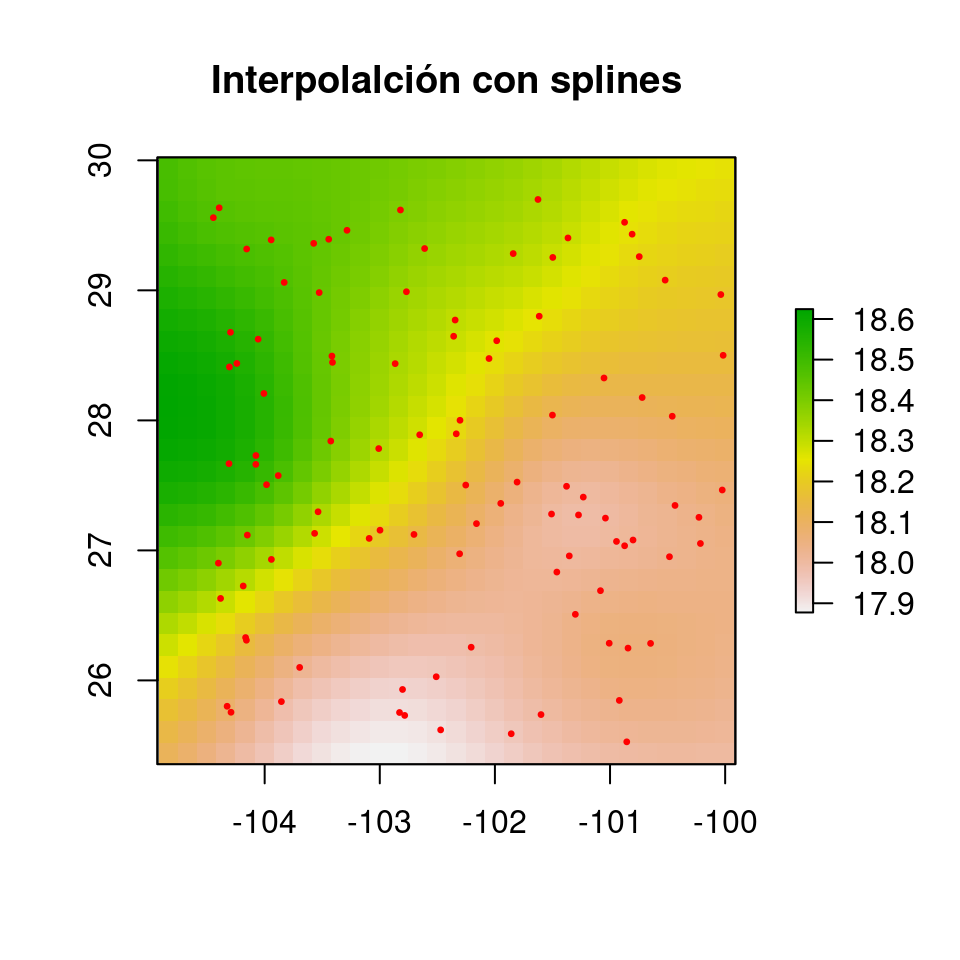
\includegraphics{Interpolacion/Splines-ejemplo.png}
\end{frame}

\end{document}
